% 2008 年福建卷理科第 6 题：长方体 ABCD-A1B1C1D1，AB=BC=2，AA1=1，
%   求 BC1 与平面 BB1D1D 所成角的正弦值。
% 来源 PDF：gaokaomath-src/普通高考/2008/2008福建理.pdf
% SHA-256：516e8ac8e113868afa9bc4af4724c3b43f22a1f7fecc830a7f3400b8d973d452
% 原页：2008福建理.pdf 第 1 页（A3 三栏）第 1 栏，书页码 441。
% 重绘依据：按原页斜投影：A 前左下、B 前右下、C 右侧、D 被遮挡；A1、B1、C1、D1 为对应顶点；
%   A—D、D—C、D—D1、B—D 虚线，其余棱与对角线 BC1 实线。
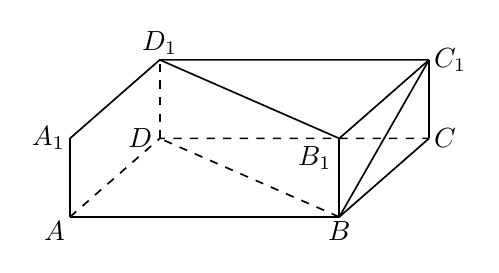
\begin{tikzpicture}[scale=0.95, semithick, every node/.style={inner sep=1.5pt}]
  \coordinate (A) at (0.00,0.00);
  \coordinate (B) at (3.60,0.00);
  \coordinate (C) at (4.80,1.05);
  \coordinate (D) at (1.20,1.05);
  \coordinate (A1) at (0.00,1.05);
  \coordinate (B1) at (3.60,1.05);
  \coordinate (C1) at (4.80,2.10);
  \coordinate (D1) at (1.20,2.10);

  \draw (A) -- (B) -- (C);
  \draw (A) -- (A1);
  \draw (B) -- (B1);
  \draw (C) -- (C1);
  \draw (A1) -- (D1) -- (C1);
  \draw (D1) -- (B1);
  \draw (B1) -- (C1);
  \draw (B) -- (C1);

  \draw[dashed] (A) -- (D) -- (C);
  \draw[dashed] (D) -- (D1);
  \draw[dashed] (B) -- (D);

  \node[below left] at (A) {$A$};
  \node[below] at (B) {$B$};
  \node[right] at (C) {$C$};
  \node[left=1pt] at (D) {$D$};
  \node[left] at (A1) {$A_1$};
  \node[below left=1pt] at (B1) {$B_1$};
  \node[right] at (C1) {$C_1$};
  \node[above] at (D1) {$D_1$};
\end{tikzpicture}
